% !TEX TS-program = pdflatex
% !TEX encoding = UTF-8 Unicode

% This is a simple template for a LaTeX document using the "article" class.
% See "book", "report", "letter" for other types of document.

\documentclass[11pt]{article} % use larger type; default would be 10pt

\usepackage[utf8]{inputenc} % set input encoding (not needed with XeLaTeX)

%%% Examples of Article customizations
% These packages are optional, depending whether you want the features they provide.
% See the LaTeX Companion or other references for full information.

%%% PAGE DIMENSIONS
\usepackage{geometry} % to change the page dimensions
\geometry{a4paper} % or letterpaper (US) or a5paper or....
% \geometry{margin=2in} % for example, change the margins to 2 inches all round
% \geometry{landscape} % set up the page for landscape
%   read geometry.pdf for detailed page layout information

\usepackage{graphicx} % support the \includegraphics command and options

% \usepackage[parfill]{parskip} % Activate to begin paragraphs with an empty line rather than an indent

%%% PACKAGES
\usepackage{booktabs} % for much better looking tables
\usepackage{array} % for better arrays (eg matrices) in maths
\usepackage{paralist} % very flexible & customisable lists (eg. enumerate/itemize, etc.)
\usepackage{verbatim} % adds environment for commenting out blocks of text & for better verbatim
\usepackage{subfig} % make it possible to include more than one captioned figure/table in a single float
% These packages are all incorporated in the memoir class to one degree or another...

%%% HEADERS & FOOTERS
\usepackage{fancyhdr} % This should be set AFTER setting up the page geometry
\pagestyle{fancy} % options: empty , plain , fancy
\renewcommand{\headrulewidth}{0pt} % customise the layout...
\lhead{}\chead{}\rhead{}
\lfoot{}\cfoot{\thepage}\rfoot{}

%%% SECTION TITLE APPEARANCE
\usepackage{sectsty}
\allsectionsfont{\sffamily\mdseries\upshape} % (See the fntguide.pdf for font help)
% (This matches ConTeXt defaults)

%%% ToC (table of contents) APPEARANCE
\usepackage[nottoc,notlof,notlot]{tocbibind} % Put the bibliography in the ToC
\usepackage[titles,subfigure]{tocloft} % Alter the style of the Table of Contents
\renewcommand{\cftsecfont}{\rmfamily\mdseries\upshape}
\renewcommand{\cftsecpagefont}{\rmfamily\mdseries\upshape} % No bold!

\usepackage{hyperref}


%%% END Article customizations

%%% The "real" document content comes below...

\title{Generating Instructions in Virtual Environments\\ as a Planning Problem}
\author{Yehuda Katz, Phil Nguyen, Peratham Wiriyathammabhum}
%\date{} % Activate to display a given date or no date (if empty),
         % otherwise the current date is printed 

\begin{document}
\maketitle

\begin{abstract}
This project aims to create a Natural Language Generation system for giving instructions in virtual world with different level of abstractions. We will try to incorporate hierarchical planner into the Potsdam Natural Language Generation systems which originally use forward search for planning.
\end{abstract}

\section{Introduction}
The Challenge on Generating Instruction in Virtual Environment (GIVE) \cite{koller2010first} is an evaluation shared task for real-time natural language generation (NLG) systems. The system objective is to guide a human instruction follower (IF) to complete a treasure-hunting task in a 3D virtual world. We put our interests into the recent version of GIVE, namely, GIVE-2.5 \cite{striegnitz2011report}. GIVE-2.5 is the second second sequel of GIVE challenge which is an identical challenge to GIVE-2 \cite{koller2010report} but was hold again for a better timing.

Users will start the 3D game from the website. First, users will download the 3D client which allows them to interact with the 3D world. Next, the client will connect to the NLG system. There are 3 evaluation worlds with different difficulties as depicted in Figure.~\ref{fig:layout}. World 1 has a simple layout and buttons are easily identified. World 2 buttons are cluttered with a lot of buttons with the same colors but the user can still refer to the room by the color of the furnitures. World 3 has a maze-like layout in one room, multiple alarm tiles in another room and several doors with a lot of plants in the last room.

\begin{figure}[hbt!]
\centering
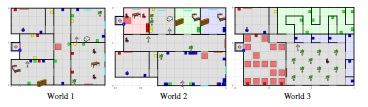
\includegraphics[width=120mm]{images/layout.jpg}
\caption{The layout of the 3 worlds in the GIVE-2.5 evaluation world \cite{striegnitz2011report}.\label{overflow}}
\label{fig:layout}
\end{figure}

The task is for a user to pick up a trophy from a safe which should be preceded by pushing a sequence of buttons. There are some obstacles such as some floor tiles that can generate an alarm signal which will cause a user to lose the game if the alarms are not deactivated in advanced. In addition, there are many unrelated objects such as lamps or plants which are dummy and will be used as landmarks by the NLG systems. The demo can be found at \url{https://www.youtube.com/watch?v=0RSin0HChno}.

The main different between GIVE and its sequels are the ability for a user to move. In GIVE, there are discrete steps so `three steps' and `turn left' will be precise actions. While in GIVE-2 and GIVE-2.5, a user can move freely so the phrases like `three steps' and `turn left' will be more difficult to predict their effects.

We are interested in the Potsdam NLG systems \cite{garoufi2011potsdam} because they use AI planning technologies for NLG. However, there are still a lot of things that can be tried. For example, the Potsdam NLG systems use Forward Search (FF). Their outputs provide just one level of abstraction. So, if hierarchical planning is used, we expect the output instructions to be more structured that will lead to the better instruction understanding.

\section{Technical Approach}

The Potsdam NLG system \cite{garoufi2011combining, garoufi2011potsdam, garoufi2014generation} is based on the previous work, the CRISP system \cite{crisp07}, which is an approach to generate natural language as a planning problem. the CRISP system can generate individual noun phrases. 

FF

Evaluation

\section{Project Management}

Task to Accomplish:
\begin{itemize}
  \item Setup the client, NLG server and the matchmaker.
  \item Understand their NLG system implementation.
  \item Make a hierarchical planner version of their NLG system.
  \item Compare the results.
\end{itemize}


\noindent
Timeline:

\begin{description}
  \item[March] \hfill \\
   Setup the client, NLG server and the matchmaker.
  \item[March] \hfill \\
  Understand their NLG system implementation.
  \item[April] \hfill \\
  Make a hierarchical planner version of their NLG system.
  \item[April] \hfill \\
  Compare the results.
  \item[May] \hfill \\
  Write summary paper.
\end{description}

\section{Conclusion}
We will try to rebuild the GIVE-2.5 challenge evaluation system. We also pick up the Potsdam NLG system which use AI planning techniques. We try to compare hierarchical planner with their conventional fast forward search (FF). 


\bibliographystyle{plain}
\bibliography{project_proposal}

\end{document}
